%!TEX root = ../thesis.tex
% ******************************* Chapter 1 appendix ********************************

\chapter{Appendix to Chapter 3}\label{appx:hivbackcalc}

\graphicspath{{02_HIVBackCalc/Figs/}}

\section{Biological markers of disease progression}\label{appendix:biomarkers}

\subsection{RITA algorithm}

The RITA algorithm defines a `recent' diagnosis as an AxSYM avidity index score less than 80.0\% or a LAg normalised optical density score less than 1.5 within 120 days of HIV diagnosis and neither of:\ a CD4 count <50 cells/mm\textsuperscript{3}, an AIDS diagnosis, nor an HIV viral load <400 copies/mL within 90 days of HIV diagnosis~\parencite{Aghaizu2014-hl}. The algorithm is shown in the flowchart in Figure~\ref{fig:rita_algorithm}.

\begin{figure}[htbp!]
  \centering
  \begin{tikzpicture}
    % Nodes
    \node[state, align=center] (r0) at (0,0) {New HIV\\diagnosis};
    \node[state, align=center] (r1) [right = 15mm of r0] {Serological test\\within 120 days};
    \node[state, align=center] (r2) [right = 15mm of r1] {Excluded};
    \node[state, align=center] (r3) [below = of r1] {Avidity <80\%\\ or LAg <1.5};
    \node[state, align=center] (r4) [right = 15mm of r3] {Not recent};
    \node[state, align=center] (r5) [below = of r3] {Treatment initiation\\before serological sample};
    \node[state, align=center] (r6) [right = 15mm of r5] {Excluded};
    \node[state, align=center] (r7) [below = of r5] {CD4 <50 cells/mm\textsuperscript{3}, \\ AIDS within 3 months,\\ or viral load <400 copies/mL};
    \node[state, align=center] (r8) [right = 15mm of r7] {Not recent};
    \node[state, align=center] (r9) [below = of r7] {Recent};
    % Edges
    \draw [->] (r0) -- (r1);
    \draw [->] (r1) -- node[above] {No} (r2);
    \draw [->] (r1) -- node[right] {Yes} (r3);
    \draw [->] (r3) -- node[above] {No} (r4);
    \draw [->] (r3) -- node[right] {Yes} (r5);
    \draw [->] (r5) -- node[above] {Yes} (r6);
    \draw [->] (r5) -- node[right] {No} (r7);
    \draw [->] (r7) -- node[above] {Yes} (r8);
    \draw [->] (r7) -- node[right] {No} (r9);
  \end{tikzpicture}
  \caption[RITA algorithm applied to EW\&NI HIV surveillance data]{RITA algorithm applied to EW\&NI HIV surveillance data.}\label{fig:rita_algorithm}
\end{figure}

\subsection{Viral load}

The HIV viral load measures the number of HIV virus copies in a millilitre of blood, expressed as copies/mL. As shown in Figure~\ref{fig:cd4dip}, in the absence of intervention, viral load measurements follow an approximately inverse pattern to the CD4 trajectory; peaking at around 100,000 copies/mL as a result of viremia during acute HIV infection, falling to a lower level post-seroconversion, then rising in late infection~\parencite{Maartens2014-xd}. With initiation of ART, HIV viral load will diminish, preventing onwards transmission of the virus~\parencite{Delpech2022-af}.

Viral loads are collected routinely at healthcare visits and, at the population level, inform measurement of the proportion of people with untransmittable levels of virus.

\subsection{p24 antigen}

The p24 HIV antigen is a viral protein which makes up the HIV viral core~\parencite{Pebody2021-wr}\@. p24 antigen levels in the blood spike during acute infection, but then subside as antibodies to p24 start to be produced the body during seroconversion. As a result, the p24 antigen is typically only detectable during early infection and p24 antigen assays alone are not a reliable way of diagnosing HIV after seroconversion.

The latest `fourth-generation' HIV diagnostic tests make use of the fact that p24 antigens are detectable in blood before HIV antibodies by combining p24 antigen and HIV antibody tests (whereas `third-generation' tests only detect HIV antibodies). Fourth-generation antibody/antigen laboratory tests are now the standard screening assay in the UK, with an estimated median window period between infection and detection of 17.8 days (IQR 13.0 to 23.6 days)~\parencite{Delaney2017-co}.

\subsection{HIV testing history}

Whilst not a strictly `biological' marker of disease progression, HIV testing history can provide useful information about an individual's likely time of HIV acquisition:\ since individuals with a previous negative HIV test must have acquired HIV in the period between the last negative and first positive test. A more recent negative test indicates a shorter window during which the infection was acquired, for example, a previous negative HIV test within 12 months could be classed as evidence of `recent' infection.

\section{Availability of biomarker data}\label{appendix:biomarker-availability}

\subsection{HIV avidity assay data}

Samples for HIV avidity assay testing are collected through sentinel surveillance from a subset of clinics. \cite{Aghaizu2018-kk} demonstrated that the population tested for avidity assays prior to 2013 were broadly representative of all EW\&NI diagnoses. To assess whether this remains true in more recent years, and in particular among GBM, all available avidity assay scores from national testing and linked to a diagnosis record were considered.

Table~\ref{tab:rita_demog} shows the demographic characteristics of GBM diagnosed in EW\&NI between 2011--2019 by avidity assay availability. Age and ethnicity characteristics were similar for GBM with and without assay results available, although avidity assay results were slightly more common among younger GBM compared to older GBM\@. Over the 14-year analysis period, diagnoses in London and Northern Ireland were over-represented for assay result availability, whilst diagnoses in Wales and the Midlands and East of England were under-represented.

\begin{table}[!h]
\centering\centering
\caption{\label{tab:rita_demog}Demographic characteristics of GBM newly diagnosed in EW\&NI between 2011--2019 by availability of incidence assay.}
\centering
\begin{tabular}[t]{lcc}
\toprule
\textbf{Characteristic} & \makecell[c]{\textbf{Assay result available}\ \ \\N = 11,653} & \makecell[c]{\textbf{Assay result not available}\ \ \\N = 8,045}\\
\midrule
Age group at diagnosis &  & \\
\hspace{1em}15-24 & 1,850 (15.9\%) & 1,205 (15.0\%)\\
\hspace{1em}25-34 & 4,533 (38.9\%) & 3,015 (37.5\%)\\
\hspace{1em}35-49 & 3,951 (33.9\%) & 2,772 (34.5\%)\\
\hspace{1em}50-64 & 1,185 (10.2\%) & 903 (11.2\%)\\
\hspace{1em}65+ & 134 (1.1\%) & 150 (1.9\%)\\
Ethnicity &  & \\
\hspace{1em}White & 9,068 (77.8\%) & 6,262 (77.8\%)\\
\hspace{1em}Black African & 316 (2.7\%) & 187 (2.3\%)\\
\hspace{1em}Black Caribbean & 236 (2.0\%) & 150 (1.9\%)\\
\hspace{1em}Black other & 133 (1.1\%) & 84 (1.0\%)\\
\hspace{1em}Asian & 703 (6.0\%) & 478 (5.9\%)\\
\hspace{1em}Other/Mixed & 906 (7.8\%) & 639 (7.9\%)\\
\hspace{1em}Not Stated & 291 (2.5\%) & 245 (3.0\%)\\
Region of residence &  & \\
\hspace{1em}London & 5,728 (49.2\%) & 3,235 (40.2\%)\\
\hspace{1em}Midlands and East of England & 1,659 (14.2\%) & 1,432 (17.8\%)\\
\hspace{1em}North of England & 2,217 (19.0\%) & 1,439 (17.9\%)\\
\hspace{1em}South of England & 1,723 (14.8\%) & 1,323 (16.4\%)\\
\hspace{1em}Northern Ireland & 282 (2.4\%) & 69 (0.9\%)\\
\hspace{1em}Wales & 44 (0.4\%) & 547 (6.8\%)\\
CD4 count at diagnosis &  & \\
\hspace{1em}<200 & 1,724 (14.8\%) & 1,139 (14.2\%)\\
\hspace{1em}200-350 & 1,965 (16.9\%) & 1,124 (14.0\%)\\
\hspace{1em}350-500 & 2,716 (23.3\%) & 1,465 (18.2\%)\\
\hspace{1em}500+ & 4,469 (38.4\%) & 2,688 (33.4\%)\\
\hspace{1em}No CD4 & 779 (6.7\%) & 1,629 (20.2\%)\\
\bottomrule
\end{tabular}
\end{table}


Figure~\ref{fig:rita_avail} panel A shows the availability of avidity assay data over time among newly diagnosed GBM, which ranged between \var{assay_avail_low}\% and \var{assay_avail_high}\% annually between 2011 and 2019.

As shown in Figure~\ref{fig:rita_avail} panel B, the CD4 profile among newly diagnosed GBM with and without an assay result available was similar for each calendar year. Diagnoses with an avidity assay result available had fewer missing CD4 counts (as in Table~\ref{tab:rita_demog}), but, where CD4 data were available, annual trends were similar regardless of the availability of avidity assay.

The RITA algorithm was applied to obtain the classification of recent or non-recent HIV acquisition (see Section~\ref{appendix:biomarkers} for details). Figure~\ref{fig:rita_avail} panel C shows trends in the proportion of diagnoses classified as recently acquired HIV each year, stratified by CD4 count at diagnosis and avidity assay. Whilst a change of avidity assay took place in 2013 (as described in Section~\ref{sec:hiv-surveillance}), the MDRI was approximately equal between the two assays (around 6 months) and similar proportions were obtained regardless of which assay was used. Trends were relatively consistent over time in each CD4 strata; for the most part the strata did not overlap, and those with a missing CD4 count appear somewhere in the middle of the range. Those with a CD4 count above 500 cells/mm\textsuperscript{3} were most likely to be diagnosed with recently acquired HIV\@. However, a sizeable proportion of diagnoses with low CD4 counts (CD4 <200 or 200--350 cells/mm\textsuperscript{3}) were also classified as recent.

Figure~\ref{fig:rita_avail} panel D shows the same proportion of diagnoses recently acquired broken down by age group. Focussing on those with low CD4 counts (CD4 <200 or 200--350 cells/mm\textsuperscript{3}), younger individuals were more likely to be classified with recently acquired HIV as compared to older individuals.
\newline

\begin{figure}[htbp!]
  \centering
  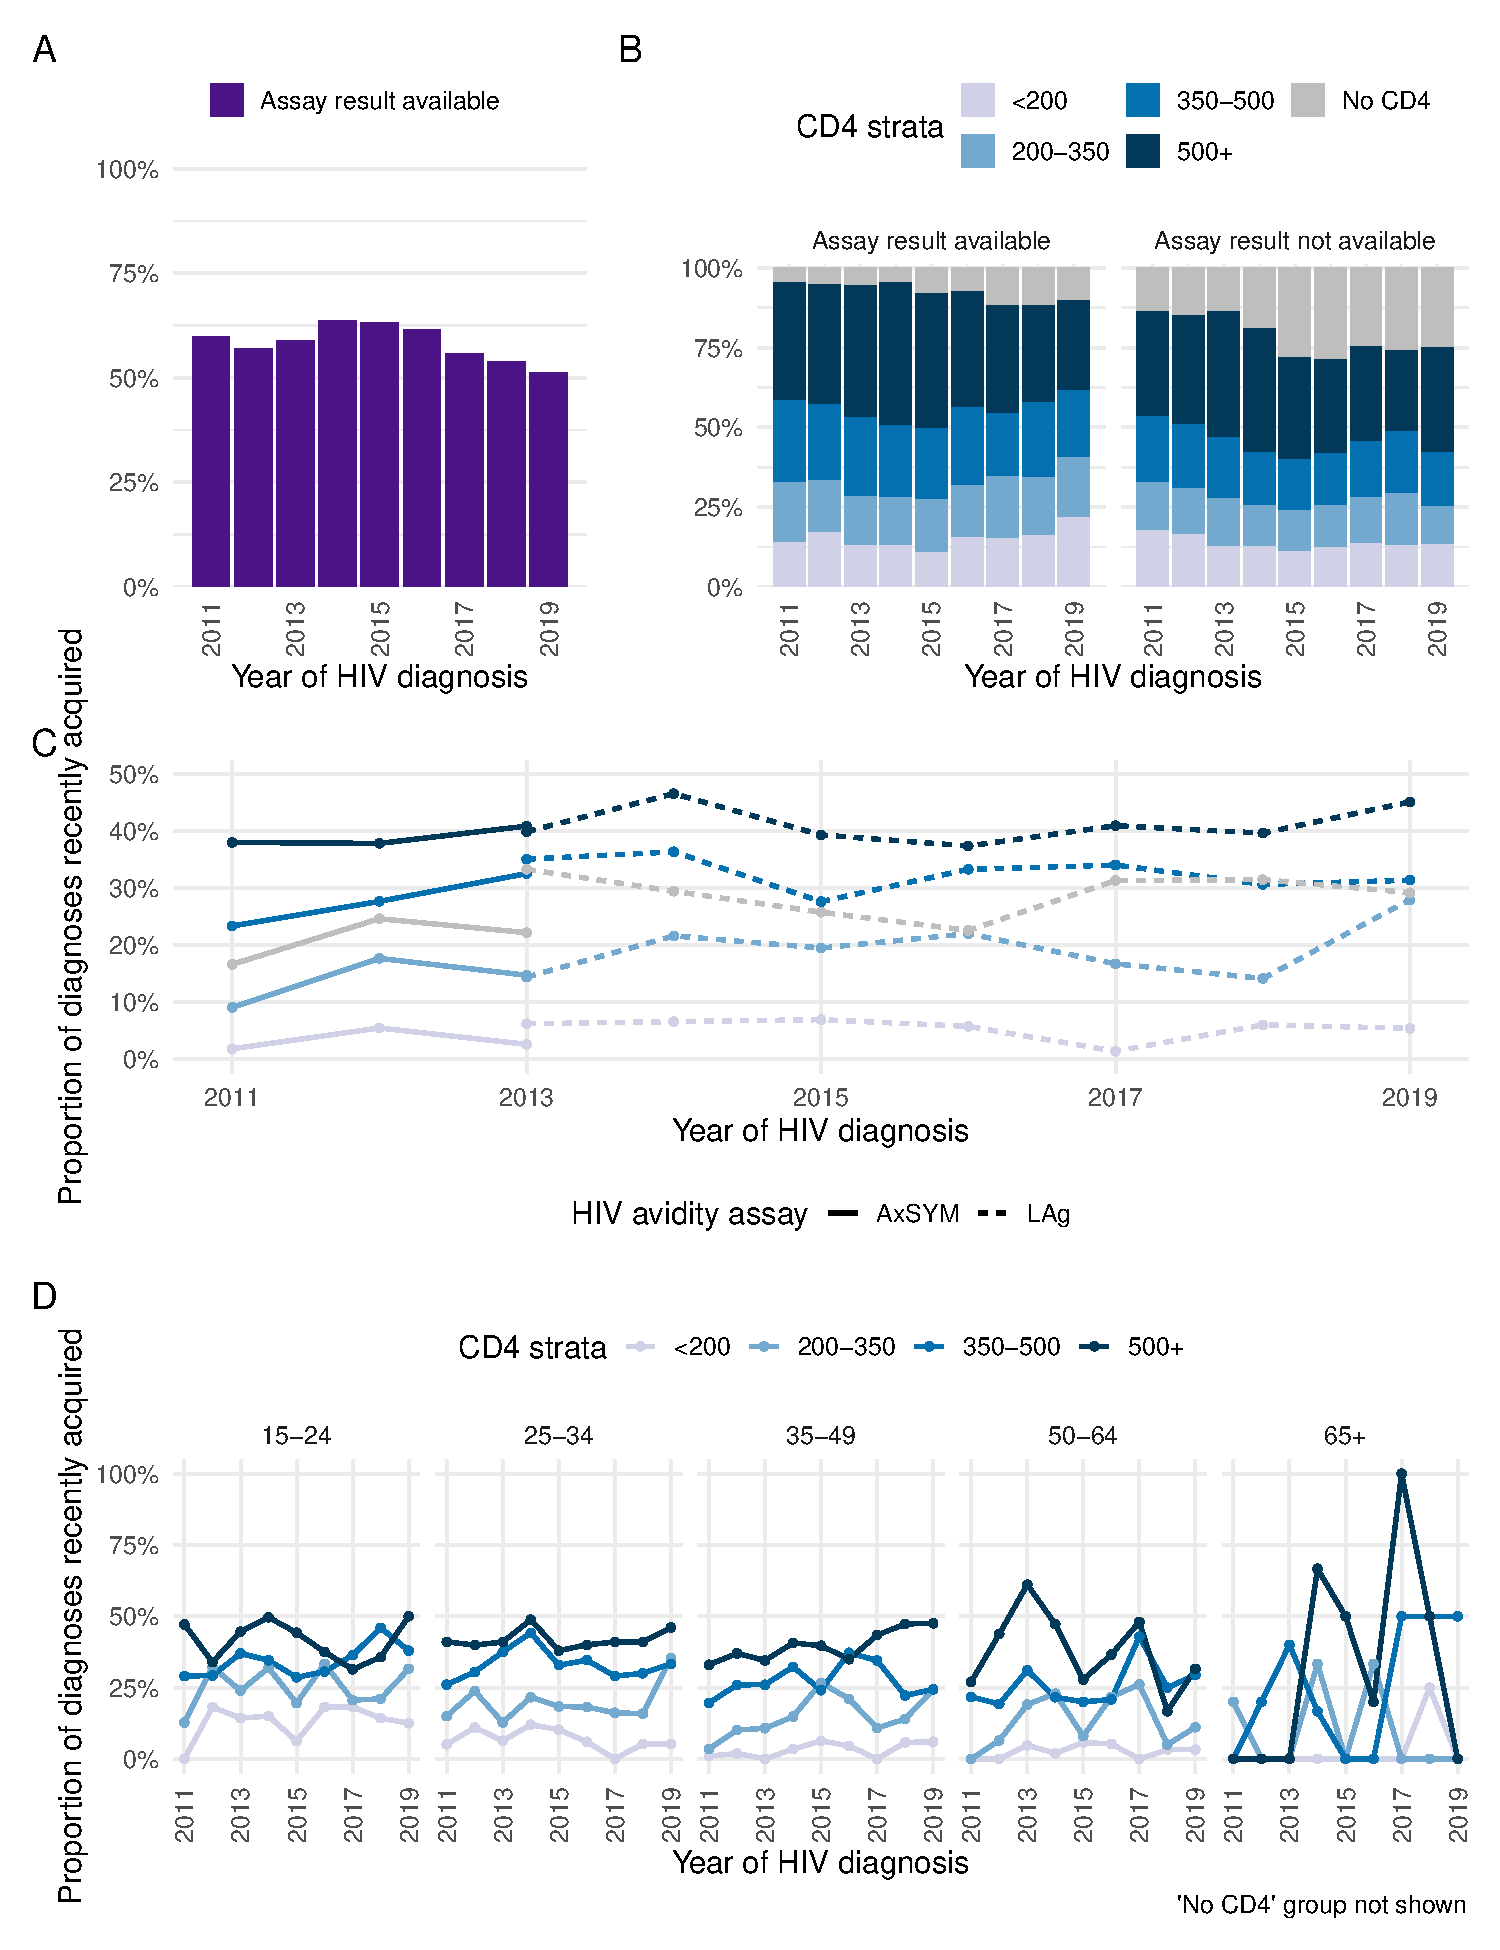
\includegraphics[width=\textwidth]{rita_availability_by_cd4.pdf}
  \caption[Availability of HIV avidity assay among GBM]{Availability of HIV avidity assay among GBM, by year of HIV diagnosis (Panel A) and CD4 count at HIV diagnosis (Panel B). Proportion of diagnoses among GBM recently acquired, by year of HIV diagnosis, CD4 count at diagnosis and avidity assay used (Panel C) and age group at HIV diagnosis (both assays combined) (Panel D).}\label{fig:rita_avail}
\end{figure}

Table~\ref{tab:cd4_dist_age} shows the overall number and proportion in each CD4 stratum, by age group, for GBM diagnosed with recently acquired HIV between 2011--2019. Whilst numbers are small for certain groups, \var{prop_cd4_1524}\% of those aged 15--24 had a CD4 count in the <200 or 200--350 cells/mm\textsuperscript{3} range compared to \var{prop_cd4_3549}\% among those aged 35--49. Table~\ref{tab:cd4_dist_eey} shows the same data, broken down by year of HIV diagnosis, demonstrating that CD4 distributions among those recently diagnosed were relatively stable over time, with smaller numbers of tests available in recent years.

\begin{table}[!h]
\centering\centering
\caption{\label{tab:cd4_dist_age}Distribution of CD4 cell counts among those diagnosed with recently acquired HIV between 2011--2019, by age group at diagnosis.}
\centering
\resizebox{\ifdim\width>\linewidth\linewidth\else\width\fi}{!}{
\begin{tabular}[t]{lcccccc}
\toprule
\multicolumn{1}{c}{ } & \multicolumn{5}{c}{Age group at diagnosis} & \multicolumn{1}{c}{ } \\
\cmidrule(l{3pt}r{3pt}){2-6}
 & 15-24 & 25-34 & 35-49 & 50-64 & 65+ & Total\\
\midrule
CD4 strata &  &  &  &  &  & \\
\hspace{1em}<200 & 16 (2.7\%) & 37 (2.7\%) & 21 (2.3\%) & 9 (4.2\%) & 1 (5.6\%) & 84 (2.7\%)\\
\hspace{1em}200-350 & 77 (13.0\%) & 146 (10.8\%) & 90 (9.9\%) & 30 (14.0\%) & 3 (16.7\%) & 346 (11.2\%)\\
\hspace{1em}350-500 & 167 (28.3\%) & 367 (27.2\%) & 236 (26.0\%) & 56 (26.2\%) & 7 (38.9\%) & 833 (27.1\%)\\
\hspace{1em}500+ & 331 (56.0\%) & 800 (59.3\%) & 559 (61.7\%) & 119 (55.6\%) & 7 (38.9\%) & 1,816 (59.0\%)\\
\bottomrule
\end{tabular}}
\end{table}


\begin{table}[!h]
\centering\centering
\caption{\label{tab:cd4_dist_eey}Distribution of CD4 cell counts among those diagnosed with recently acquired HIV between 2011--2019, by year of diagnosis.}
\centering
\begin{tabular}[t]{lcccc}
\toprule
\multicolumn{1}{c}{ } & \multicolumn{4}{c}{CD4 strata} \\
\cmidrule(l{3pt}r{3pt}){2-5}
 & <200 & 200-350 & 350-500 & 500+\\
\midrule
Year of diagnosis &  &  &  & \\
\hspace{1em}2011 & 4 (1.2\%) & 26 (7.8\%) & 91 (27.2\%) & 213 (63.8\%)\\
\hspace{1em}2012 & 15 (3.9\%) & 45 (11.7\%) & 102 (26.6\%) & 222 (57.8\%)\\
\hspace{1em}2013 & 8 (1.8\%) & 36 (8.1\%) & 133 (29.8\%) & 270 (60.4\%)\\
\hspace{1em}2014 & 16 (2.6\%) & 60 (9.9\%) & 150 (24.6\%) & 383 (62.9\%)\\
\hspace{1em}2015 & 12 (2.9\%) & 51 (12.1\%) & 98 (23.3\%) & 259 (61.7\%)\\
\hspace{1em}2016 & 11 (3.5\%) & 43 (13.7\%) & 97 (31.0\%) & 162 (51.8\%)\\
\hspace{1em}2017 & 2 (0.9\%) & 29 (13.4\%) & 60 (27.8\%) & 125 (57.9\%)\\
\hspace{1em}2018 & 8 (4.3\%) & 21 (11.4\%) & 58 (31.4\%) & 98 (53.0\%)\\
\hspace{1em}2019 & 8 (4.7\%) & 35 (20.5\%) & 44 (25.7\%) & 84 (49.1\%)\\
Total & 84 (2.7\%) & 346 (11.2\%) & 833 (27.1\%) & 1,816 (59.0\%)\\
\bottomrule
\end{tabular}
\end{table}


\subsection{HIV testing history data}

HIV testing history information, in particular the date of a previous negative HIV test, are directly collected through HARS whilst records of STI clinic activity (visits and tests) are monitored through the genitourinary medicine clinic activity dataset (GUMCAD)\nomenclature[z]{GUMCAD}{Genitourinary medicine clinic activity dataset}. These data represent upper bounds on the time since HIV acquisition for an individual, so whilst a last negative test within 6 months may indicate recent acquisition, the lack of such a result is not an indication of longstanding infection.

HIV testing history was available for a subset of diagnosed individuals and for this analysis, all available last negative HIV test results from HARS and GUMCAD which had been linked to a subsequent HIV diagnosis record for GBM in EW\&NI were considered.

Table~\ref{tab:lastneg_demog} shows the demographic characteristics of newly diagnosed GBM by previous negative test availability. Previous negative tests were more commonly available for younger GBM compared to older GBM, and those with White, Black Caribbean, and Black other ethnicity were more likely to have a previous test reported compared to other ethnicities. Previous test availability was higher among those resident in the South of England compared to other regions in England, and substantially lower in Wales and Northern Ireland. Previous negative tests were also much less common among those with a CD4 count at diagnosis <200 cells/mm\textsuperscript{3}.

\begin{table}[!h]
\centering\centering
\caption{\label{tab:lastneg_demog}Demographic characteristics of GBM newly diagnosed in EW\&NI between 2011--2019 by availability of previous negative test.}
\centering
\begin{tabular}[t]{lcc}
\toprule
\textbf{Characteristic} & \makecell[c]{\textbf{Previous negative test}\ \ \\N = 10,524} & \makecell[c]{\textbf{No previous negative test}\ \ \\N = 9,174}\\
\midrule
Age group at diagnosis &  & \\
\hspace{1em}15-24 & 1,675 (15.9\%) & 1,380 (15.0\%)\\
\hspace{1em}25-34 & 4,224 (40.1\%) & 3,324 (36.2\%)\\
\hspace{1em}35-49 & 3,609 (34.3\%) & 3,114 (33.9\%)\\
\hspace{1em}50-64 & 914 (8.7\%) & 1,174 (12.8\%)\\
\hspace{1em}65+ & 102 (1.0\%) & 182 (2.0\%)\\
Ethnicity &  & \\
\hspace{1em}White & 8,300 (78.9\%) & 7,030 (76.6\%)\\
\hspace{1em}Black African & 263 (2.5\%) & 240 (2.6\%)\\
\hspace{1em}Black Caribbean & 232 (2.2\%) & 154 (1.7\%)\\
\hspace{1em}Black other & 123 (1.2\%) & 94 (1.0\%)\\
\hspace{1em}Asian & 560 (5.3\%) & 621 (6.8\%)\\
\hspace{1em}Other/Mixed & 812 (7.7\%) & 733 (8.0\%)\\
\hspace{1em}Not Stated & 234 (2.2\%) & 302 (3.3\%)\\
Region of residence &  & \\
\hspace{1em}London & 4,774 (45.4\%) & 4,189 (45.7\%)\\
\hspace{1em}Midlands and East of England & 1,613 (15.3\%) & 1,478 (16.1\%)\\
\hspace{1em}North of England & 1,992 (18.9\%) & 1,664 (18.1\%)\\
\hspace{1em}South of England & 1,826 (17.4\%) & 1,220 (13.3\%)\\
\hspace{1em}Northern Ireland & 87 (0.8\%) & 264 (2.9\%)\\
\hspace{1em}Wales & 232 (2.2\%) & 359 (3.9\%)\\
CD4 count at diagnosis &  & \\
\hspace{1em}<200 & 1,058 (10.1\%) & 1,805 (19.7\%)\\
\hspace{1em}200-350 & 1,693 (16.1\%) & 1,396 (15.2\%)\\
\hspace{1em}350-500 & 2,505 (23.8\%) & 1,676 (18.3\%)\\
\hspace{1em}500+ & 4,268 (40.6\%) & 2,889 (31.5\%)\\
\hspace{1em}No CD4 & 1,000 (9.5\%) & 1,408 (15.3\%)\\
\bottomrule
\end{tabular}
\end{table}


Figure~\ref{fig:ln_avail} panel A shows the availability of HIV testing history over time for GBM newly diagnosed with HIV between 1995 and 2019. The proportion with information on HIV testing history available rose from 24\% in 1995 to a peak of 60\% in 2015, falling somewhat in subsequent years. A corresponding peak in the proportion with a negative test within the past 6 months was seen in 2015 (22\% of newly diagnosed GBM). Temporal trends were similar across all age groups, with a greater proportion of younger GBM having HIV testing history available compared to older GBM (Figure~\ref{fig:ln_avail} panel B).

Figure~\ref{fig:ln_avail} panel C presents the proportion with a previous negative test within 6 months by age group and CD4 count at diagnosis, between 2011--2019. A recent negative test within the past 6 months was less common among HIV diagnoses with a CD4 count <200 cells/mm\textsuperscript{3}, consistent across all age groups, with some overlap for the other CD4 strata.

\begin{figure}[htbp!]
  \centering
  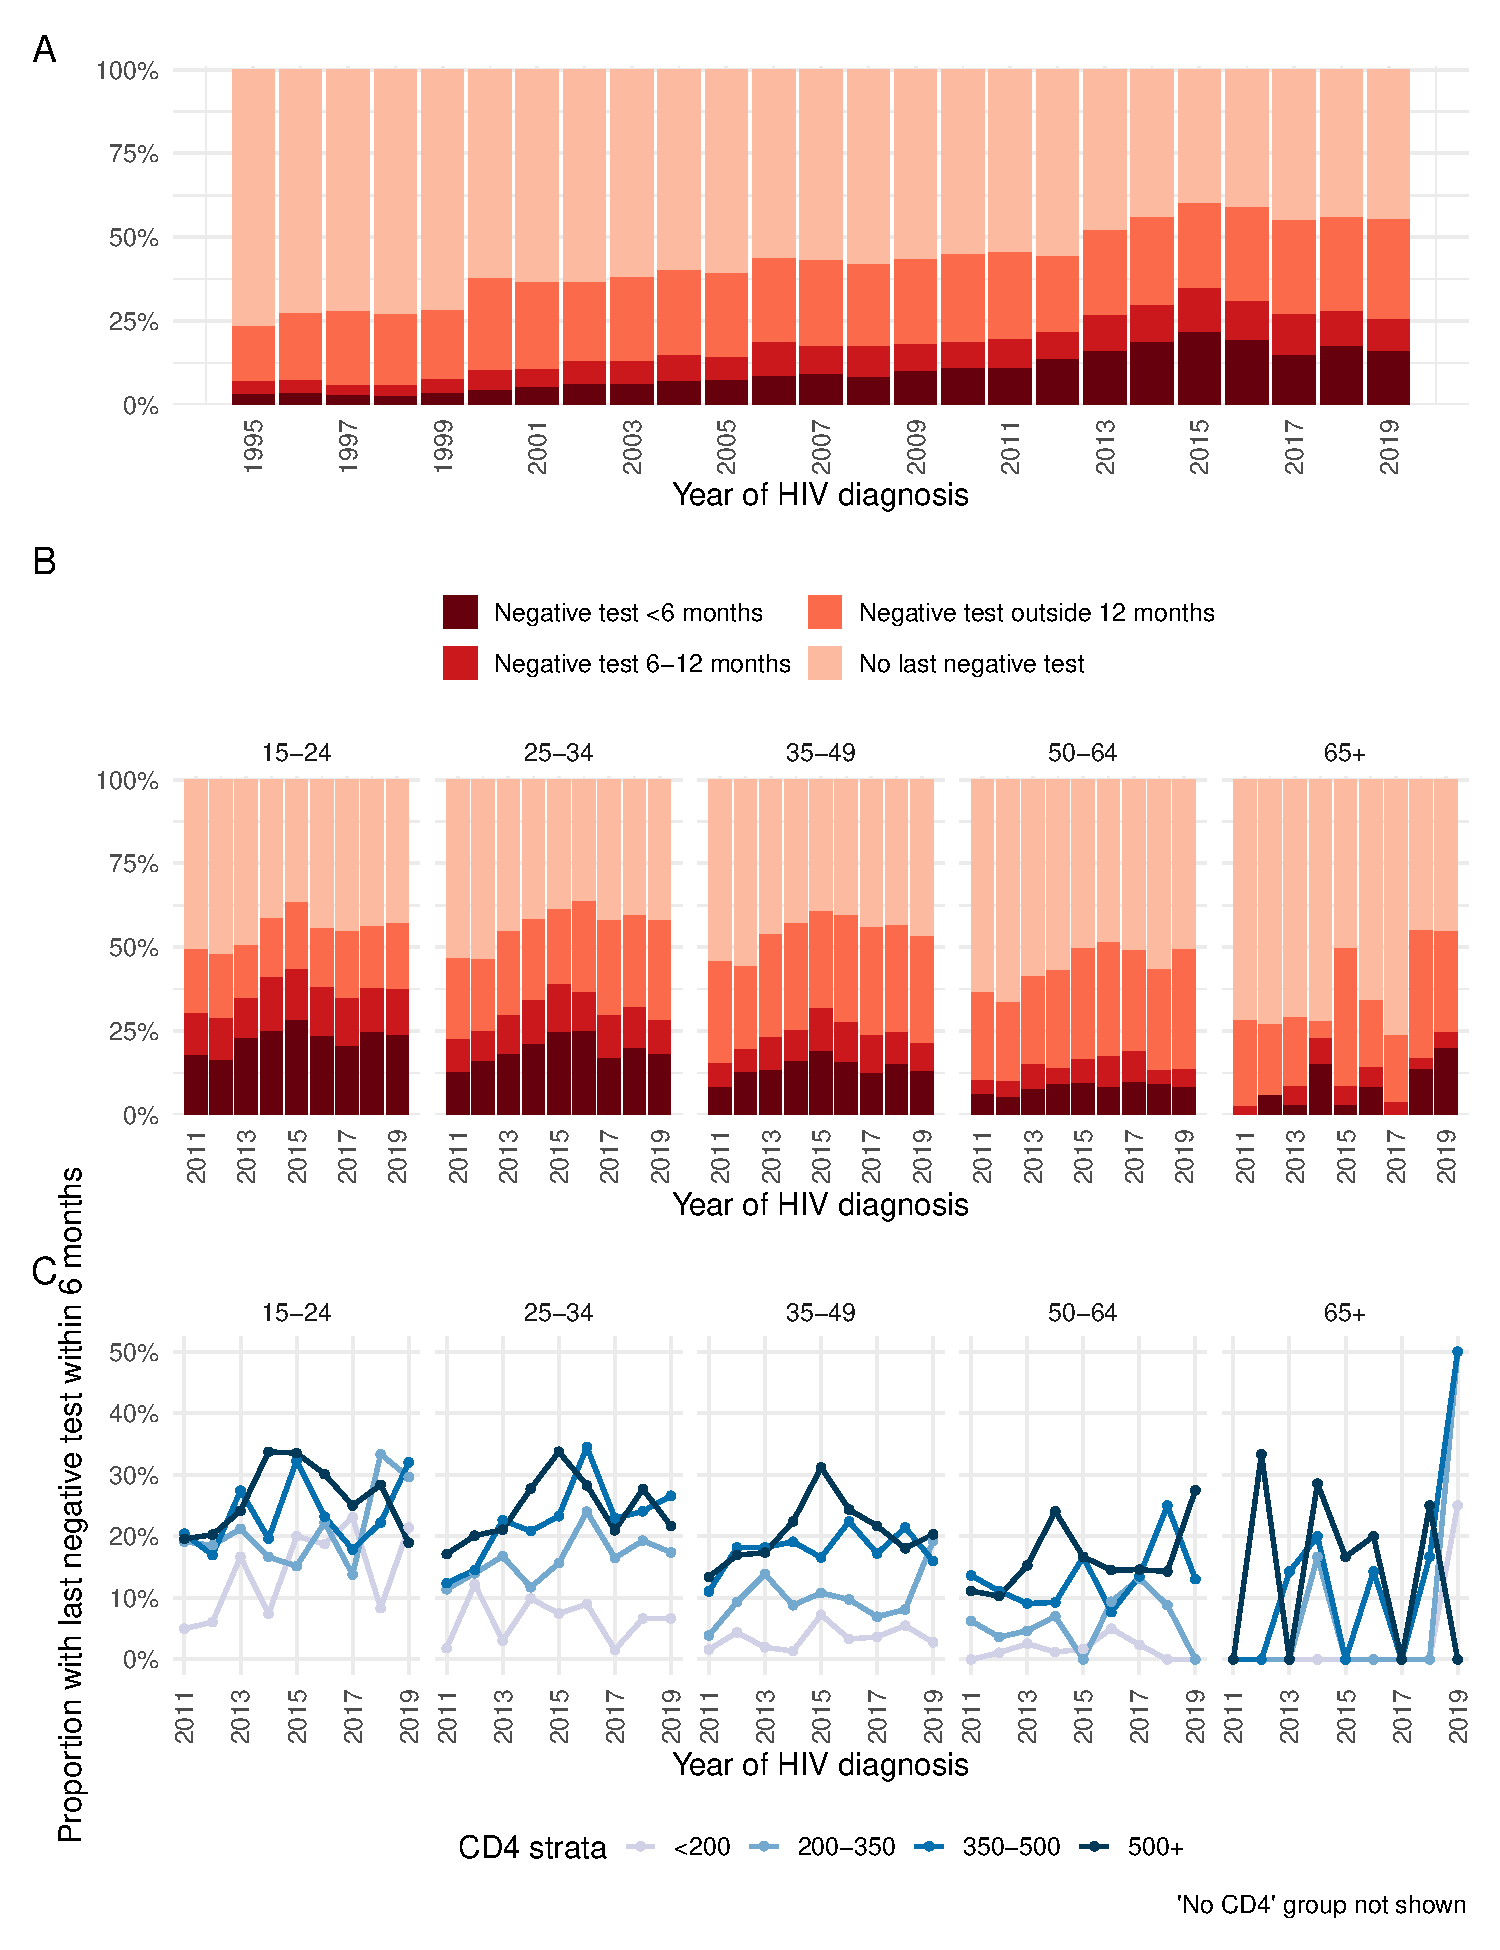
\includegraphics[width=\textwidth]{lntest_by_cd4.pdf}
  \caption[Time since last negative HIV test among GBM, by year of HIV diagnosis]{Time since last negative HIV test among GBM, by year of HIV diagnosis (Panel A), and stratified by age group at HIV diagnosis (Panel B). Proportion of HIV diagnoses with a recent test within past 6 months, stratified by CD4 count and age group at diagnosis (Panel C).}\label{fig:ln_avail}
\end{figure}

\subsection{Viral load data}

A high viral load and low CD4 count are present in both early and late presentation of HIV, as in Figure~\ref{fig:cd4dip}, therefore baseline HIV viral load information cannot be used to identify individuals with evidence of recent HIV acquisition. When taken in conjunction with other biomarkers, however, a high viral load may provide supporting evidence of diagnosis occurring during early infection.

Baseline HIV viral load data are reported for the majority of new HIV diagnoses, with additional information available via linkage to HARS\@. For this analysis, only viral loads taken within 91 days of an initial diagnosis were considered and, where treatment start date information was available, any viral loads taken post-treatment initiation were excluded.

Table~\ref{tab:vl_demog} shows the demographic characteristics of GBM newly diagnosed with and without baseline HIV viral load (VL)\nomenclature[z]{VL}{Viral load} information available. Viral load availability was similar by age and ethnicity, with some regional differences in data availability (higher in the South of England and Northern Ireland, lower in London). Where CD4 count data was missing, a baseline viral load was also much more likely to be unavailable.

\begin{table}[!h]
\centering\centering
\caption{\label{tab:vl_demog}Demographic characteristics of GBM newly diagnosed in EW\&NI between 2011--2019 by availability of baseline VL.}
\centering
\begin{tabular}[t]{lcc}
\toprule
\textbf{Characteristic} & \makecell[c]{\textbf{Baseline VL available}\ \ \\N = 12,313} & \makecell[c]{\textbf{Baseline VL not available}\ \ \\N = 7,385}\\
\midrule
Age group at diagnosis &  & \\
\hspace{1em}15-24 & 1,957 (15.9\%) & 1,098 (14.9\%)\\
\hspace{1em}25-34 & 4,693 (38.1\%) & 2,855 (38.7\%)\\
\hspace{1em}35-49 & 4,138 (33.6\%) & 2,585 (35.0\%)\\
\hspace{1em}50-64 & 1,350 (11.0\%) & 738 (10.0\%)\\
\hspace{1em}65+ & 175 (1.4\%) & 109 (1.5\%)\\
Ethnicity &  & \\
\hspace{1em}White & 9,756 (79.2\%) & 5,574 (75.5\%)\\
\hspace{1em}Black African & 298 (2.4\%) & 205 (2.8\%)\\
\hspace{1em}Black Caribbean & 232 (1.9\%) & 154 (2.1\%)\\
\hspace{1em}Black other & 135 (1.1\%) & 82 (1.1\%)\\
\hspace{1em}Asian & 744 (6.0\%) & 437 (5.9\%)\\
\hspace{1em}Other/Mixed & 901 (7.3\%) & 644 (8.7\%)\\
\hspace{1em}Not Stated & 247 (2.0\%) & 289 (3.9\%)\\
Region of residence &  & \\
\hspace{1em}London & 4,912 (39.9\%) & 4,051 (54.9\%)\\
\hspace{1em}Midlands and East of England & 2,106 (17.1\%) & 985 (13.3\%)\\
\hspace{1em}North of England & 2,518 (20.4\%) & 1,138 (15.4\%)\\
\hspace{1em}South of England & 2,176 (17.7\%) & 870 (11.8\%)\\
\hspace{1em}Northern Ireland & 245 (2.0\%) & 106 (1.4\%)\\
\hspace{1em}Wales & 356 (2.9\%) & 235 (3.2\%)\\
CD4 count at diagnosis &  & \\
\hspace{1em}<200 & 1,990 (16.2\%) & 873 (11.8\%)\\
\hspace{1em}200-350 & 2,193 (17.8\%) & 896 (12.1\%)\\
\hspace{1em}350-500 & 2,946 (23.9\%) & 1,235 (16.7\%)\\
\hspace{1em}500+ & 4,980 (40.4\%) & 2,177 (29.5\%)\\
\hspace{1em}No CD4 & 204 (1.7\%) & 2,204 (29.8\%)\\
\bottomrule
\end{tabular}
\end{table}


Figure~\ref{fig:vl_cd4_recent} panel A shows baseline viral load information among newly diagnosed GBM according to RITA classification. Across all CD4 strata, the distribution of baseline viral load was markedly different among those classified as recent compared to non-recent diagnoses. This difference was partly due to viral loads <400 copies/mL being explicitly excluded from the RITA algorithm, but also as a much higher proportion of recently acquired HIV were diagnosed with a viral load above 100,000 copies/mL.

Figure~\ref{fig:vl_cd4_recent} panel B shows baseline viral load by time since previous negative HIV test (panel B). Again those with a more recent negative test were more likely to have a baseline viral load above 100,000 copies/mL. However, the differences in baseline viral load by testing history were less marked than according to RITA classification.
\newline
\newline

\begin{figure}[htbp!]
  \centering
  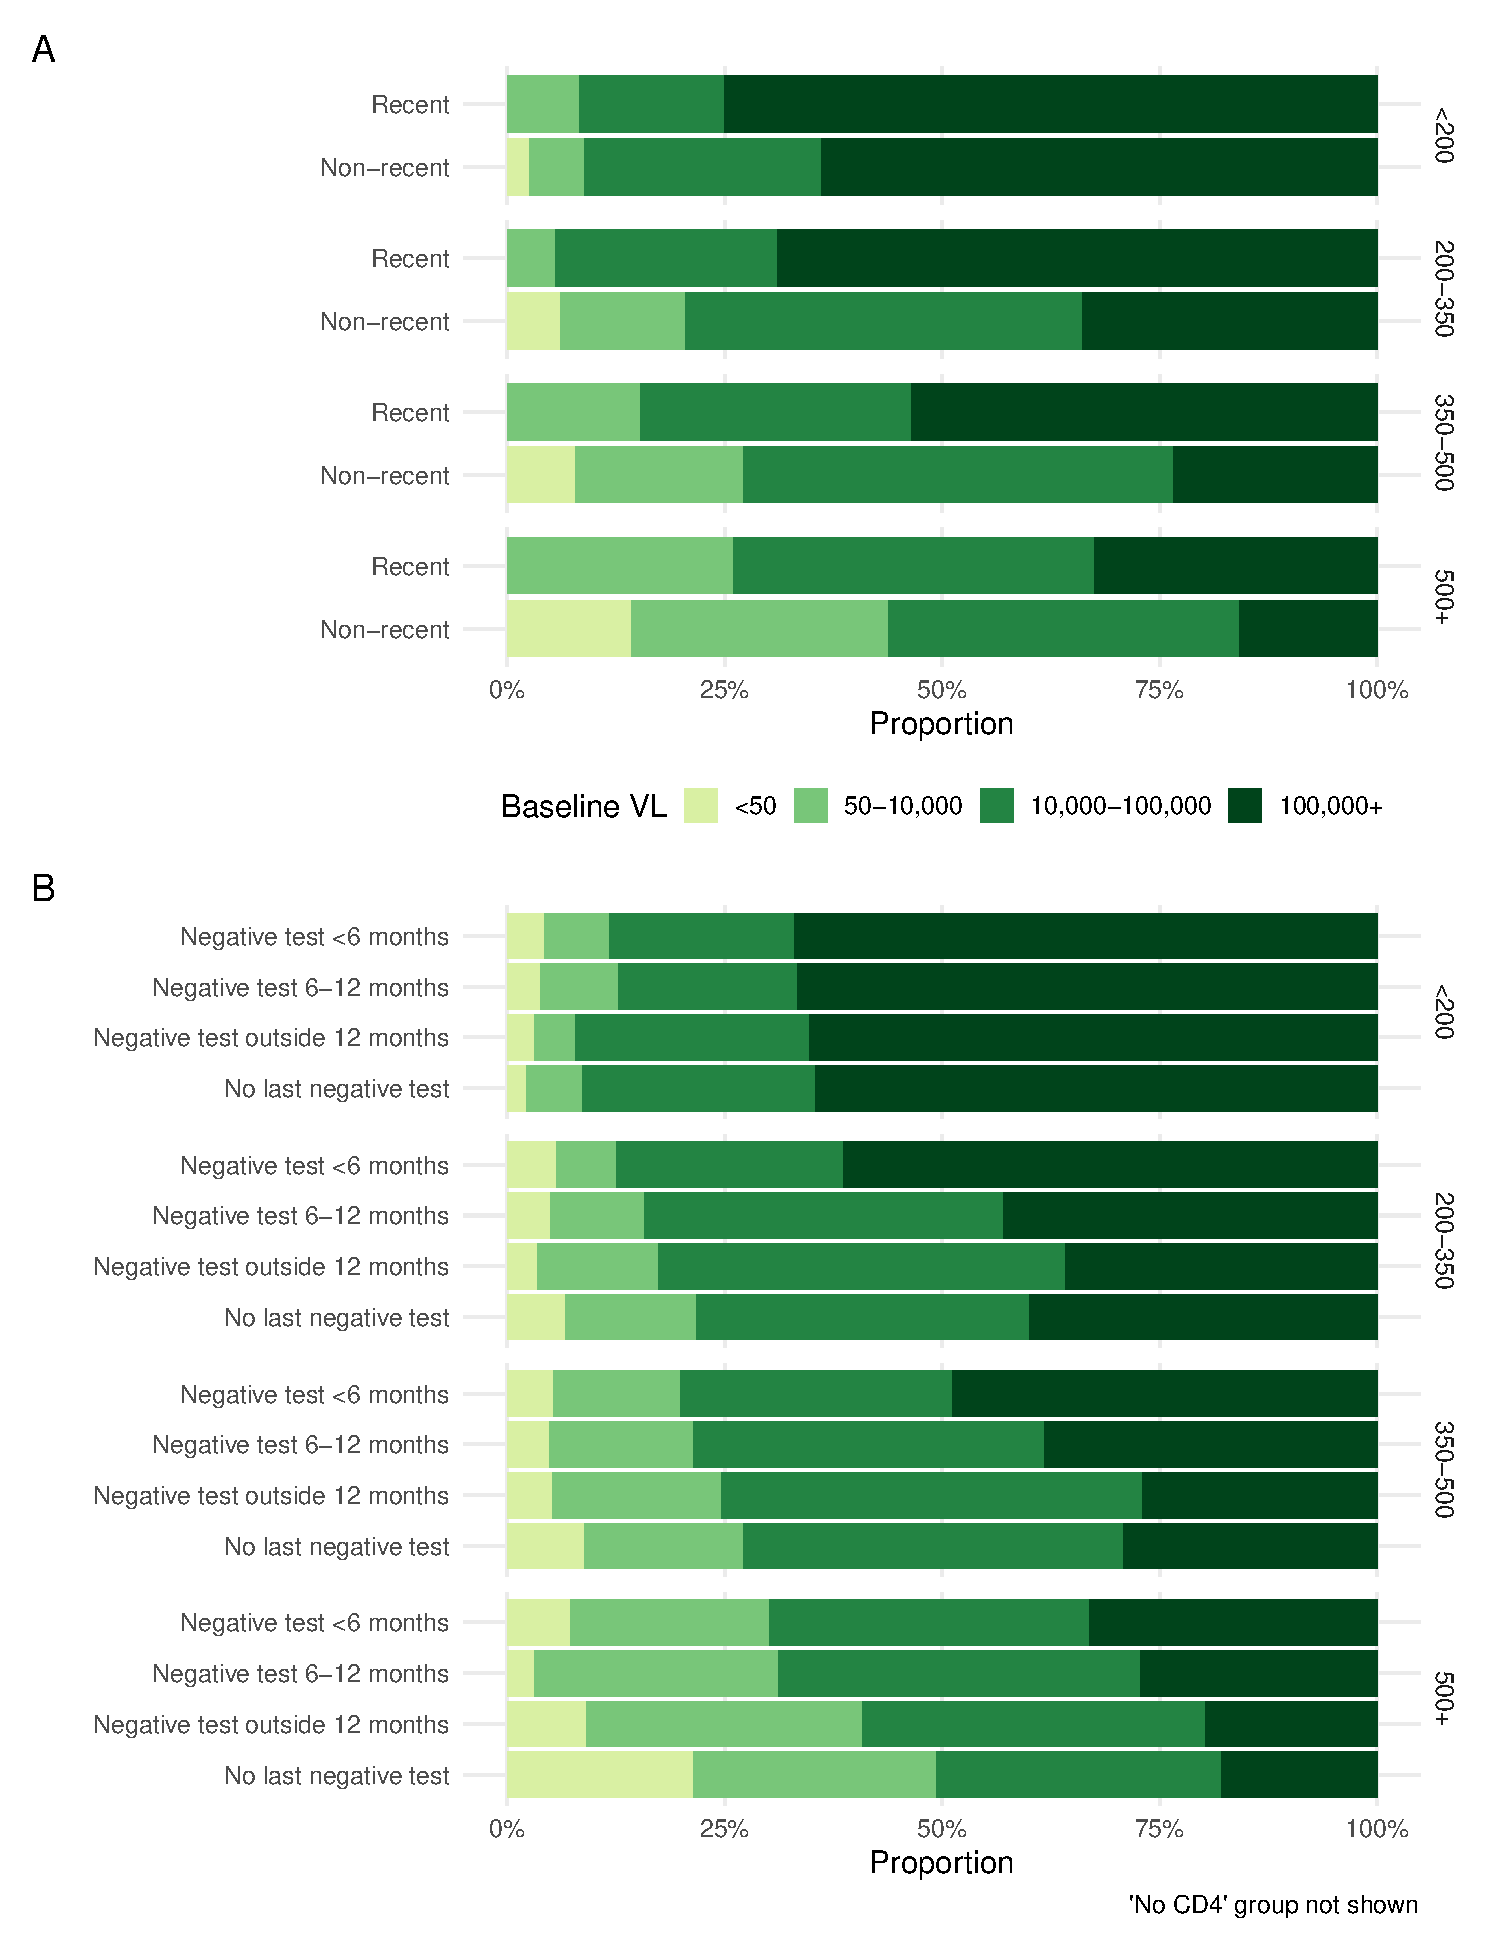
\includegraphics[width=\textwidth]{vl_cd4_recent.pdf}
  \caption[Baseline HIV viral load and CD4 strata among GBM, by avidity assay and time since previous negative test]{Baseline HIV viral load and CD4 strata among GBM, by avidity assay and time since previous negative test.}\label{fig:vl_cd4_recent}
\end{figure}

Figure~\ref{fig:vl_avail} panel A shows baseline viral load availability between 2011--2019, which has remained around 60\% over this period. Figure~\ref{fig:vl_avail} panel B demonstrates the lower completion of CD4 data among diagnoses with missing baseline viral load information, particularly after 2015. Figure~\ref{fig:vl_avail} panel C shows baseline viral load by age group and CD4 strata. Higher baseline viral load was seen for lower CD4 strata, e.g.\ a greater proportion with a viral load above 100,000 copies/mL in the CD4 <200 cells/mm\textsuperscript{3} stratum. Examined by age group, older individuals tended to have a higher baseline viral load at HIV diagnosis, regardless of CD4 strata. For more recent diagnosis, an increasing proportion had a baseline viral load <50 copies/mL, particularly in the CD4 >500 cells/mm\textsuperscript{3} stratum (Figure~\ref{fig:vl_avail} panel D).

\begin{figure}[htbp!]
  \centering
  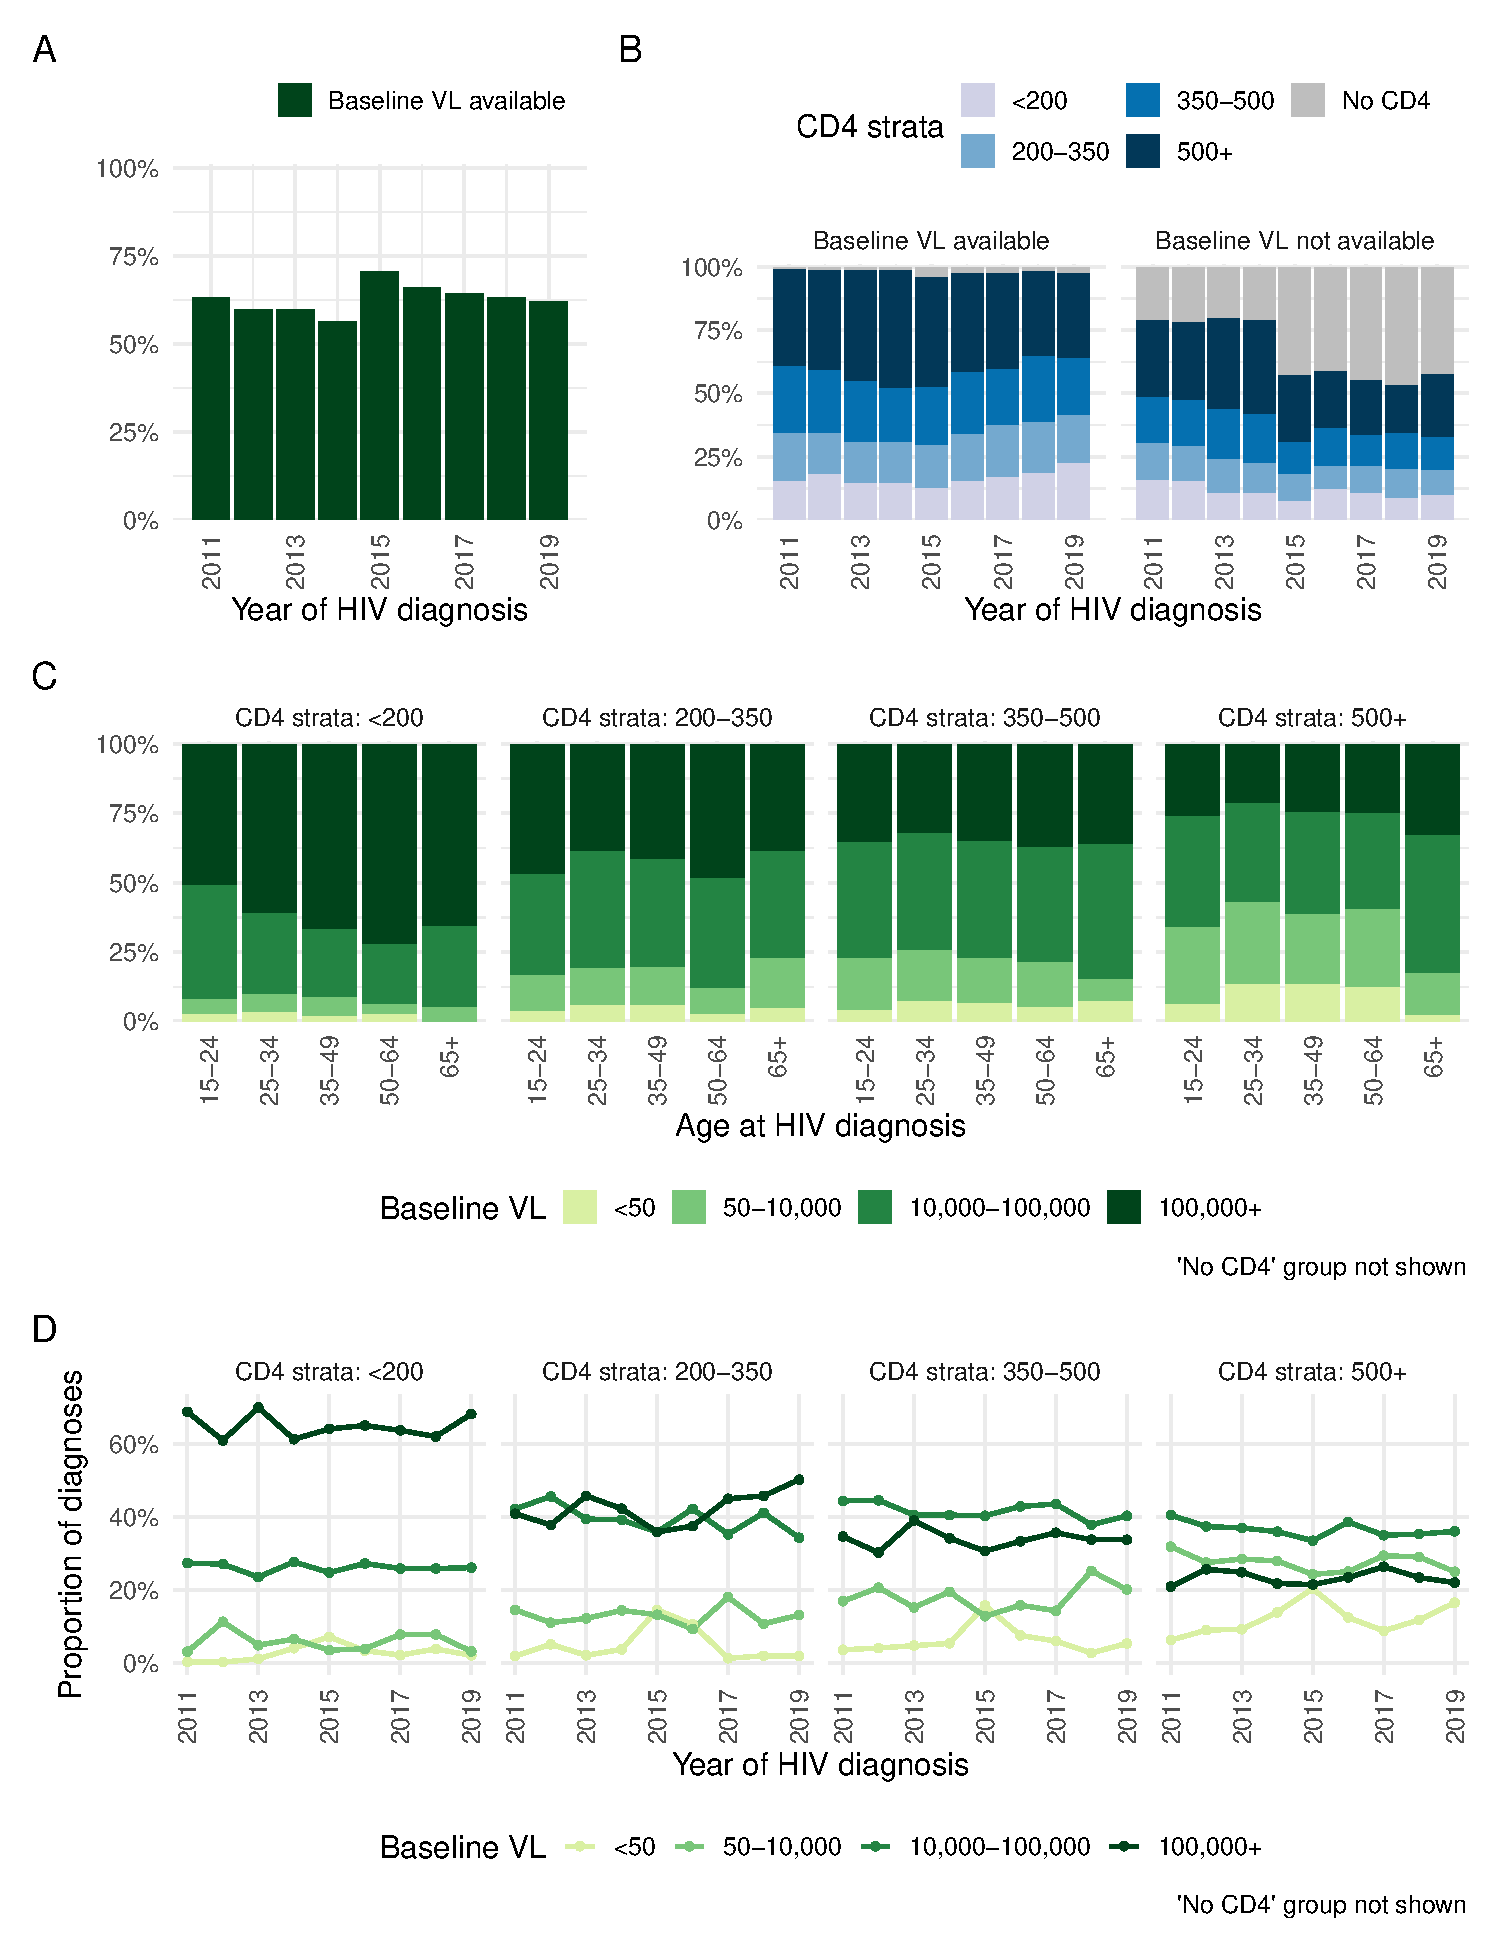
\includegraphics[scale=0.6]{vl_availability_by_cd4.pdf}
  \caption[Availability of HIV viral load among GBM]{Availability of baseline HIV viral load (VL) among GBM, by year of HIV diagnosis (Panel A) and CD4 count at HIV diagnosis (Panel B). Baseline VL among GBM by year of HIV diagnosis and age group (Panel C), and by CD4 cell count at diagnosis (Panel D).}\label{fig:vl_avail}
\end{figure}

\section{Revised late HIV diagnosis definition}\label{appendix:late-diag}

For the reclassification method for late HIV diagnosis, a correction factor (CF)\nomenclature[z]{CF}{Correction factor} was defined as the percentage change in the late HIV diagnosis rate after reclassification of individuals with evidence of recent HIV acquisition\parencite{Kirwan2022-za}:
%
\[
  \text{correction factor} =  \frac{\text{number with CD4 <350 cells/mm\textsuperscript{3} reclassified as `not late'}}{\text{number with CD4 count <350 cells/mm\textsuperscript{3}}}
\]

In 2019, across all newly diagnosed individuals in EW\&NI, reclassification for recent infection resulted in a downwards adjustment of the late diagnosis rate by 14\%. This was highest among GBM (26\% in 2019), particularly younger GBM (CF of 46\% for those aged 15--24 years) and those living in London (CF 30\%). Figure~\ref{fig:latediag} panel A shows the proportion of individuals diagnosed with a CD4 $\geq$350 cells/mm\textsuperscript{3} and CD4 <350 cells/mm\textsuperscript{3}, by reclassification and probable route of HIV exposure. The evidence used to reclassify is shown in Figure~\ref{fig:latediag} panel B.

Risk factors for reclassification included exposure through sex between men and a younger age at diagnosis. The refined definition of late HIV diagnosis was shown to focus the late diagnosis measure on those at greatest risk of death.

\begin{figure}[htbp!]
  \centering
  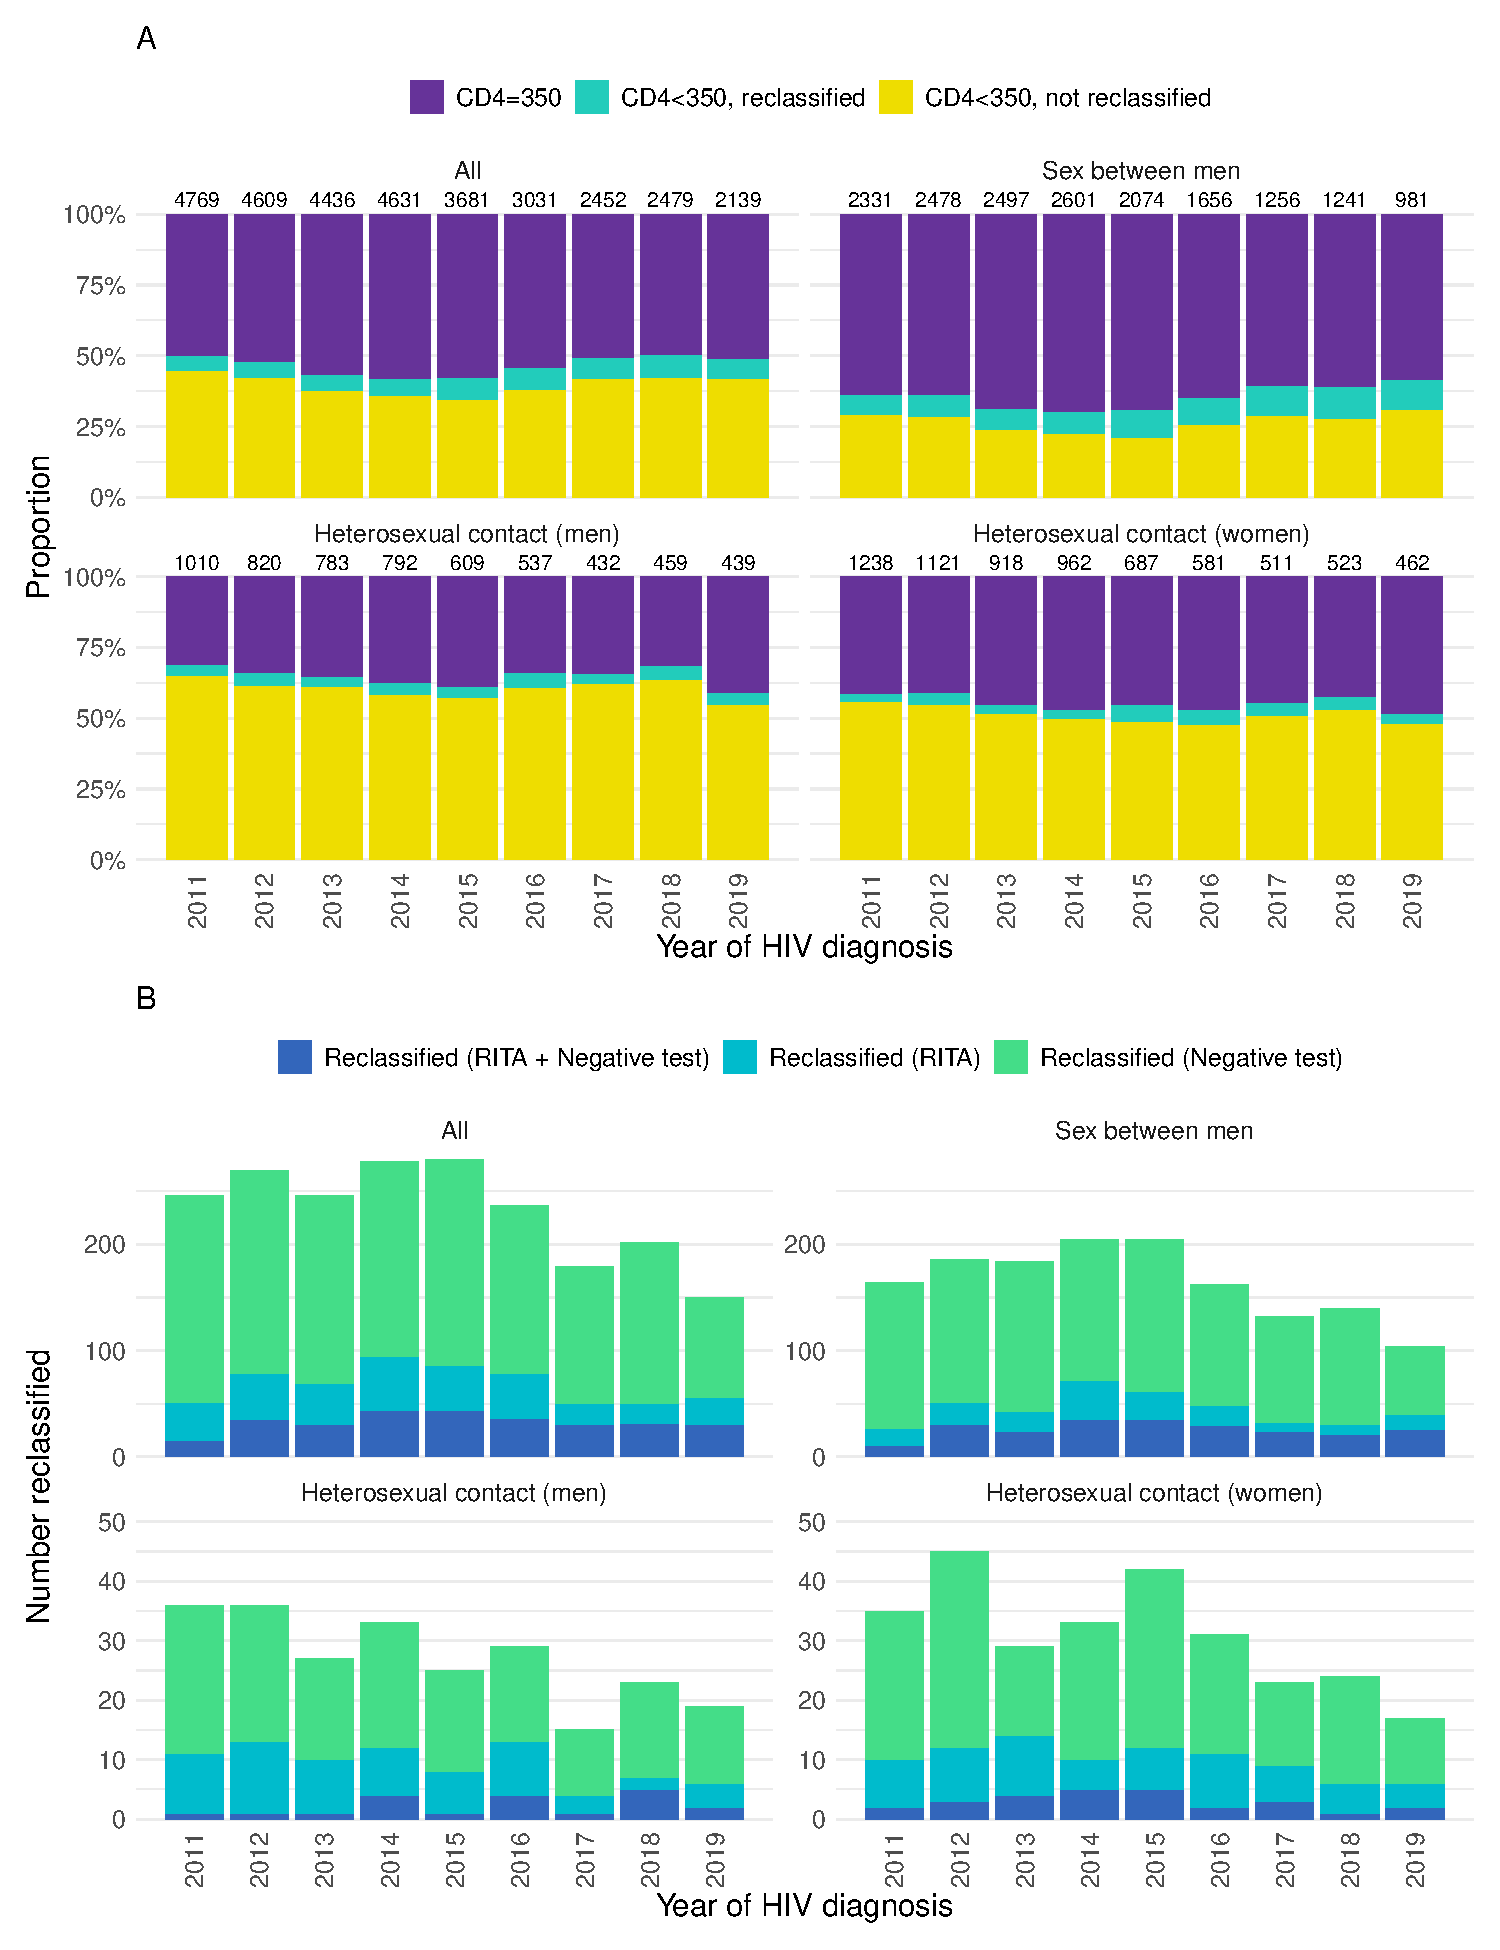
\includegraphics[width=\textwidth]{latediag.pdf}
  \caption[HIV diagnoses by re-classification and reason for re-classification]{HIV diagnoses by year of HIV diagnosis, route of HIV exposure, CD4 count, re-classification (Panel A) and reason for re-classification (Panel B). Total number of diagnoses by year and exposure group shown at top of bar in Panel A. RITA:\ recent infection testing algorithm.}\label{fig:latediag}
\end{figure}

\section{CD4 reclassification model}\label{appendix:naivereclassify}

This section presents the results of the CD4-only back-calculation model fitted to the datasets simulated in scenario (iii), in which recent diagnoses were reclassified to the CD4 500+ stratum (as described in Section~\ref{sec:hiv-simulation}).

The estimates obtained from this model were very similar to the dual biomarker model, with overlapping trends in estimated incidence and undiagnosed prevalence in Figure~\ref{fig:sim_estimates_reclass}, and the PMSE was comparable between the two models (Figure~\ref{fig:boxplot_reclass}).

\begin{figure}
  \centering
  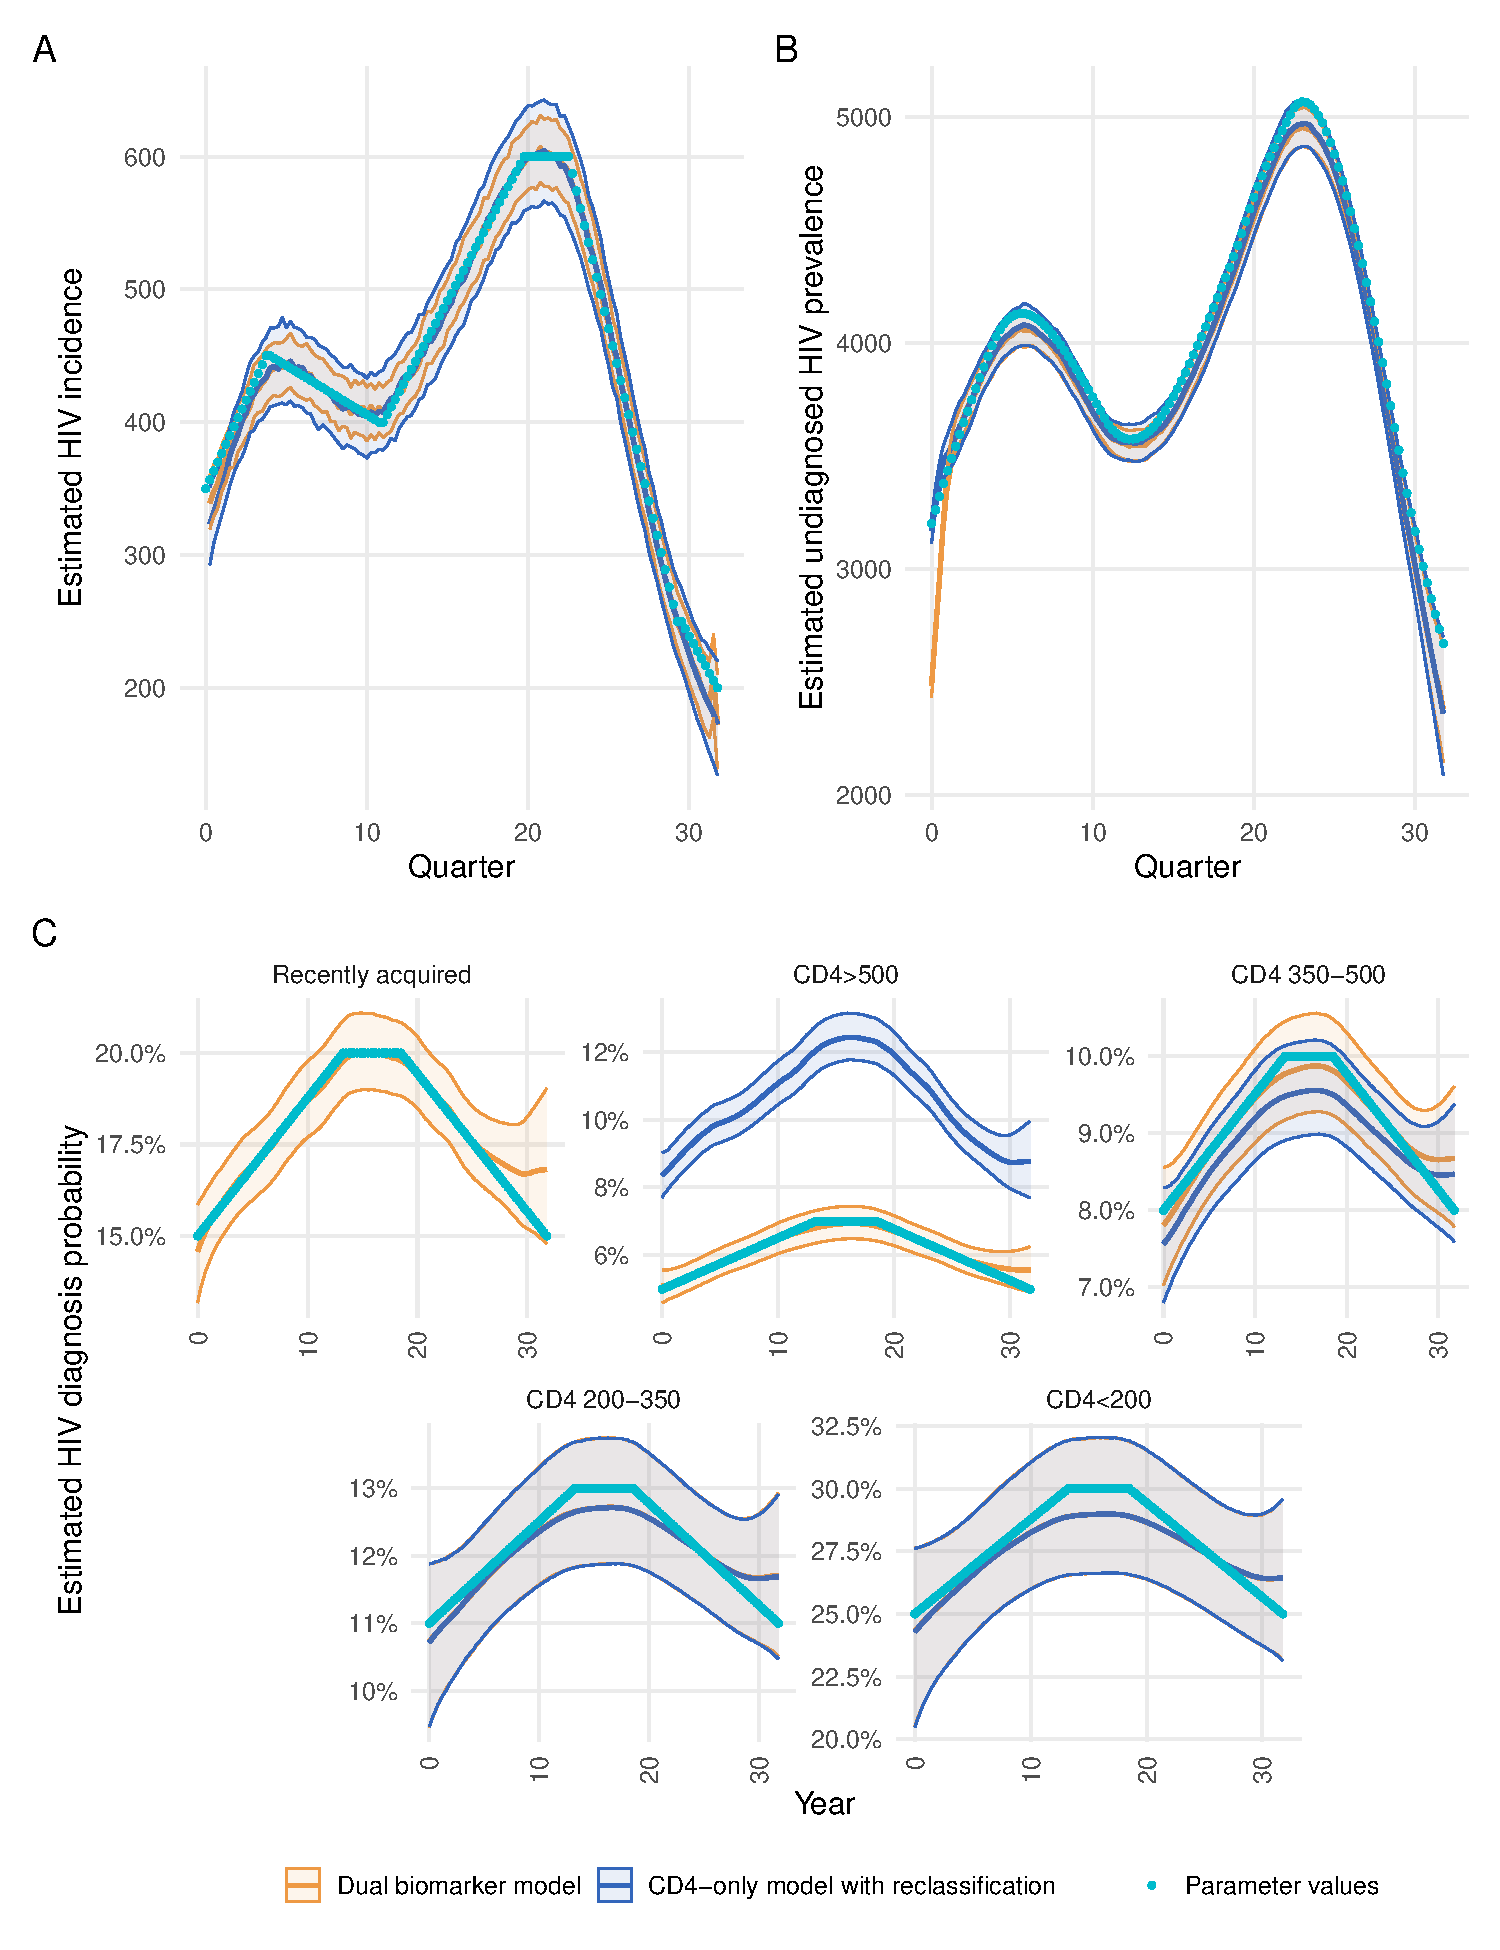
\includegraphics[width=\textwidth]{sim_estimates_reclass.pdf}
  \caption[Estimated posterior median and 95\% CrI of HIV incidence, undiagnosed prevalence, and diagnosis probabilities]{Estimated posterior median and 95\% CrI of HIV incidence, undiagnosed prevalence, and diagnosis probabilities, averaged over 100 model fits, compared to simulated data.}\label{fig:sim_estimates_reclass}
\end{figure}

\begin{figure}
  \centering
  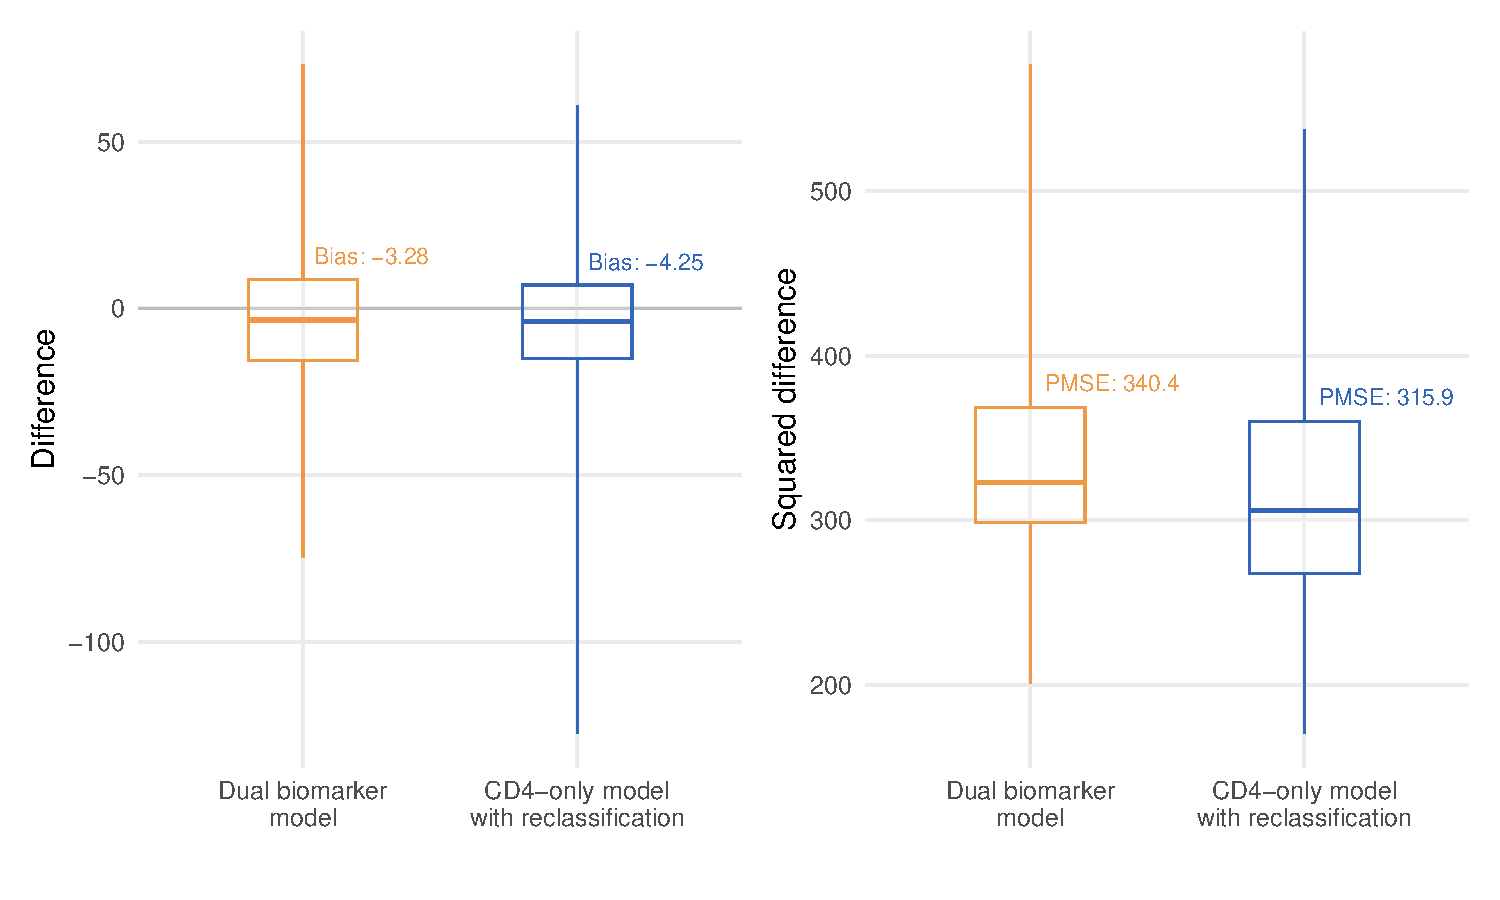
\includegraphics[width=\textwidth]{incidence_mse_reclass.pdf}
  \caption[Distributions of differences and squared differences between parameter value and estimated HIV incidence, by back-calculation model]{Distributions of differences (panel A), and squared differences (panel B) between parameter value and estimated HIV incidence, by back-calculation model. Estimates from 100 model fits. Boxplots show median, inter-quartile range, and range of estimates for each model.}\label{fig:boxplot_reclass}
\end{figure}

\section{Simulation performance with missing information}\label{appendix:simmissing}

This section presents the results of the dual biomarker and CD4-only back-calculation models fitted to simulated data scenarios (i) and (ii) with 40\% missing CD4 and RITA information (as described in Section~\ref{sec:hiv-simulation}).

The missing information made little difference to the median estimates, as shown in Figure~\ref{fig:sim_estimates_miss}. Again the PMSE was lower for the dual biomarker model compared to the CD4-only model (Figure~\ref{fig:boxplot_miss}).

\begin{figure}
  \centering
  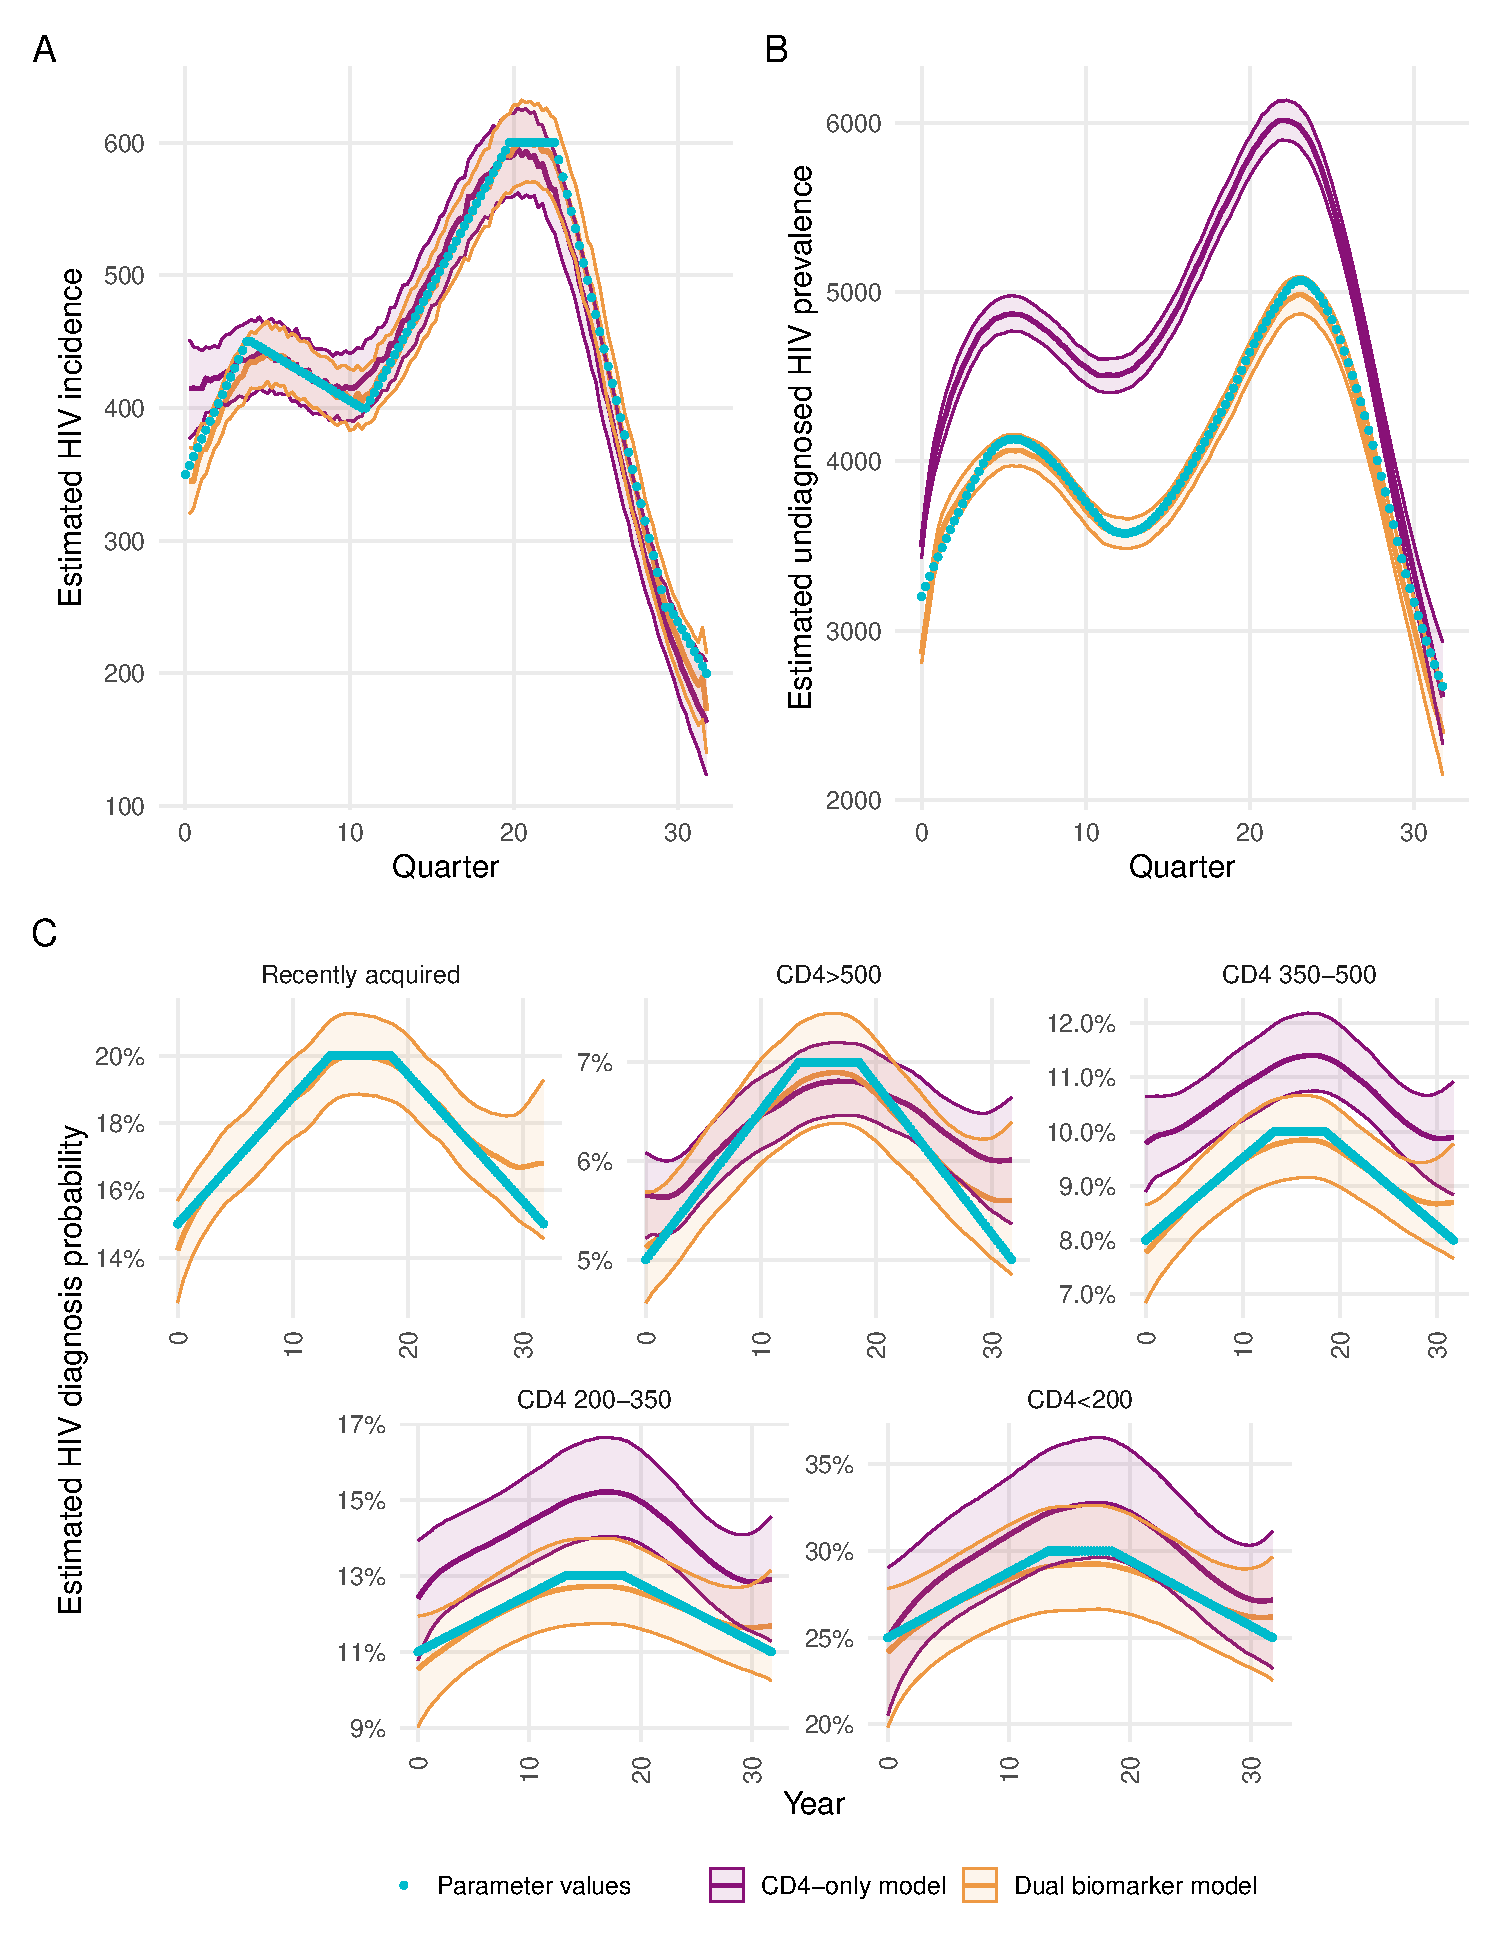
\includegraphics[width=\textwidth]{sim_estimates_miss.pdf}
  \caption[Estimated posterior median and 95\% CrI of HIV incidence, undiagnosed prevalence, and diagnosis probabilities]{Estimated posterior median and 95\% CrI of HIV incidence, undiagnosed prevalence, and diagnosis probabilities, averaged over 100 model fits, compared to simulated data. 40\% of records in simulated data missing CD4 and RITA information.}\label{fig:sim_estimates_miss}
\end{figure}

\begin{figure}
  \centering
  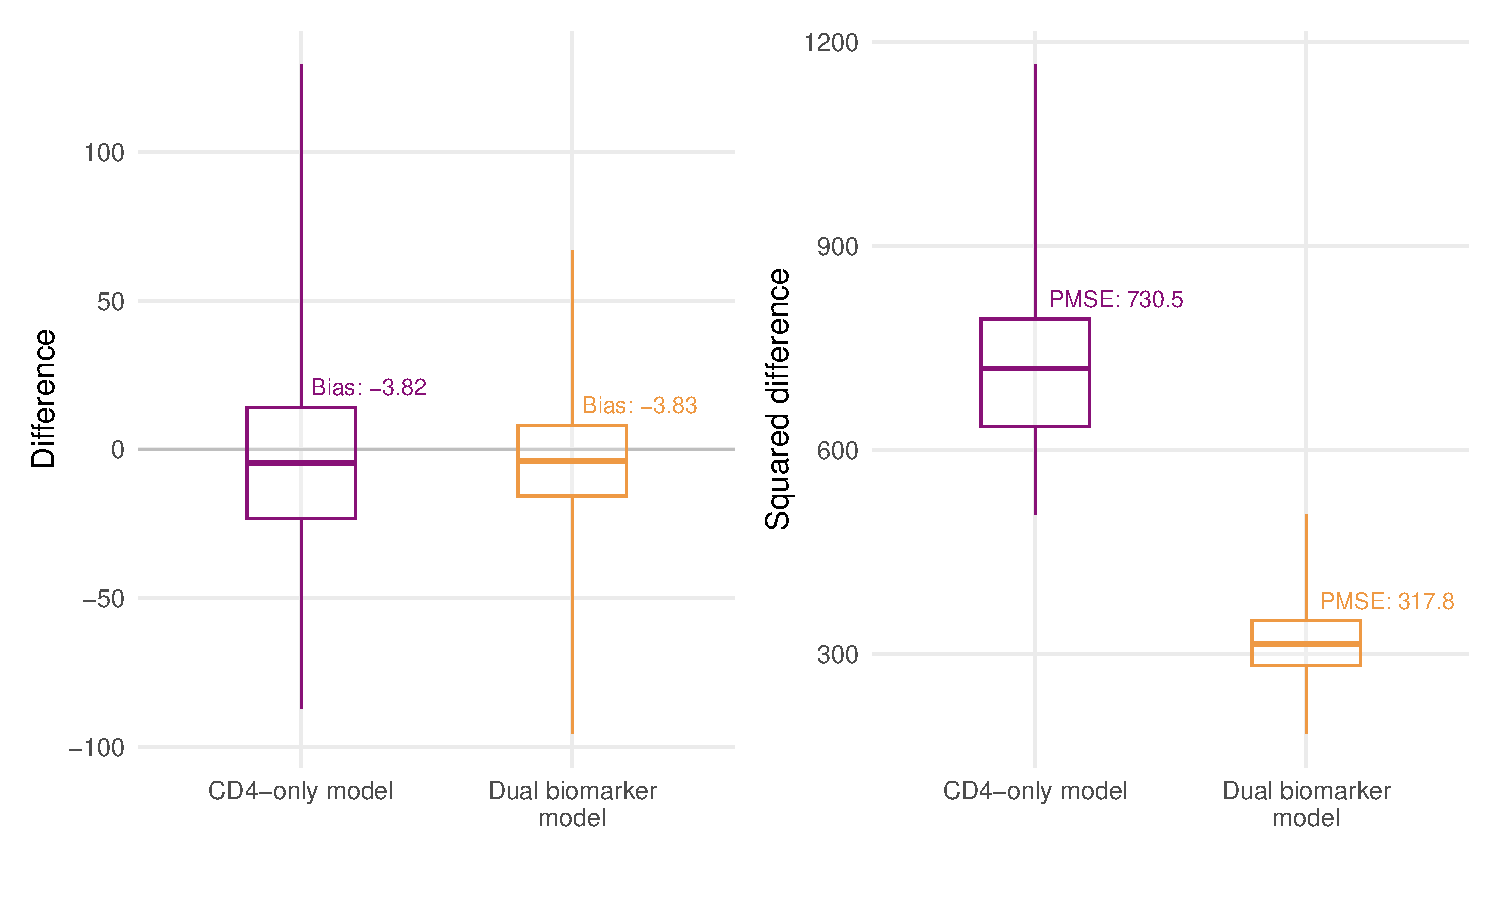
\includegraphics[width=\textwidth]{incidence_mse_miss.pdf}
  \caption[Distributions of differences and squared differences between parameter value and estimated HIV incidence, by back-calculation model]{Distributions of differences (panel A), and squared differences (panel B) between parameter value and estimated HIV incidence, by back-calculation model. Estimates from 100 model fits. 40\% of records in simulated data missing CD4 and RITA information. Boxplots show median, inter-quartile range, and range of estimates for each model.}\label{fig:boxplot_miss}
\end{figure}
